\chapter{案例计算分析和可靠性分析}\label{ch:案例计算分析和可靠性分析}


\section{案例展示}\label{sec:案例展示}
由于多条最短路算法的复杂性,在大规模图中使用手工试算来求解几乎是不可能的,因此作者实现了一个专门用于求解多条最短路的程序。下面将通过对一个简单的检测图分别进行手工计算和程序处理来检测程序设计的正确性。以计算图 17中的3条最短路为例进行算法设计的具体说明。


\section{算法执行流程}\label{sec:算法执行流程}
\begin{enumerate}%:列表
    \item 执行Dijkstra单源最短路算法求得最短路径$A^1$,如图\ref{fig:fig18}所示
    \begin{figure}[H] %H为当前位置,!htb为忽略美学标准,htbp为浮动图形
        \centering %图片居中
        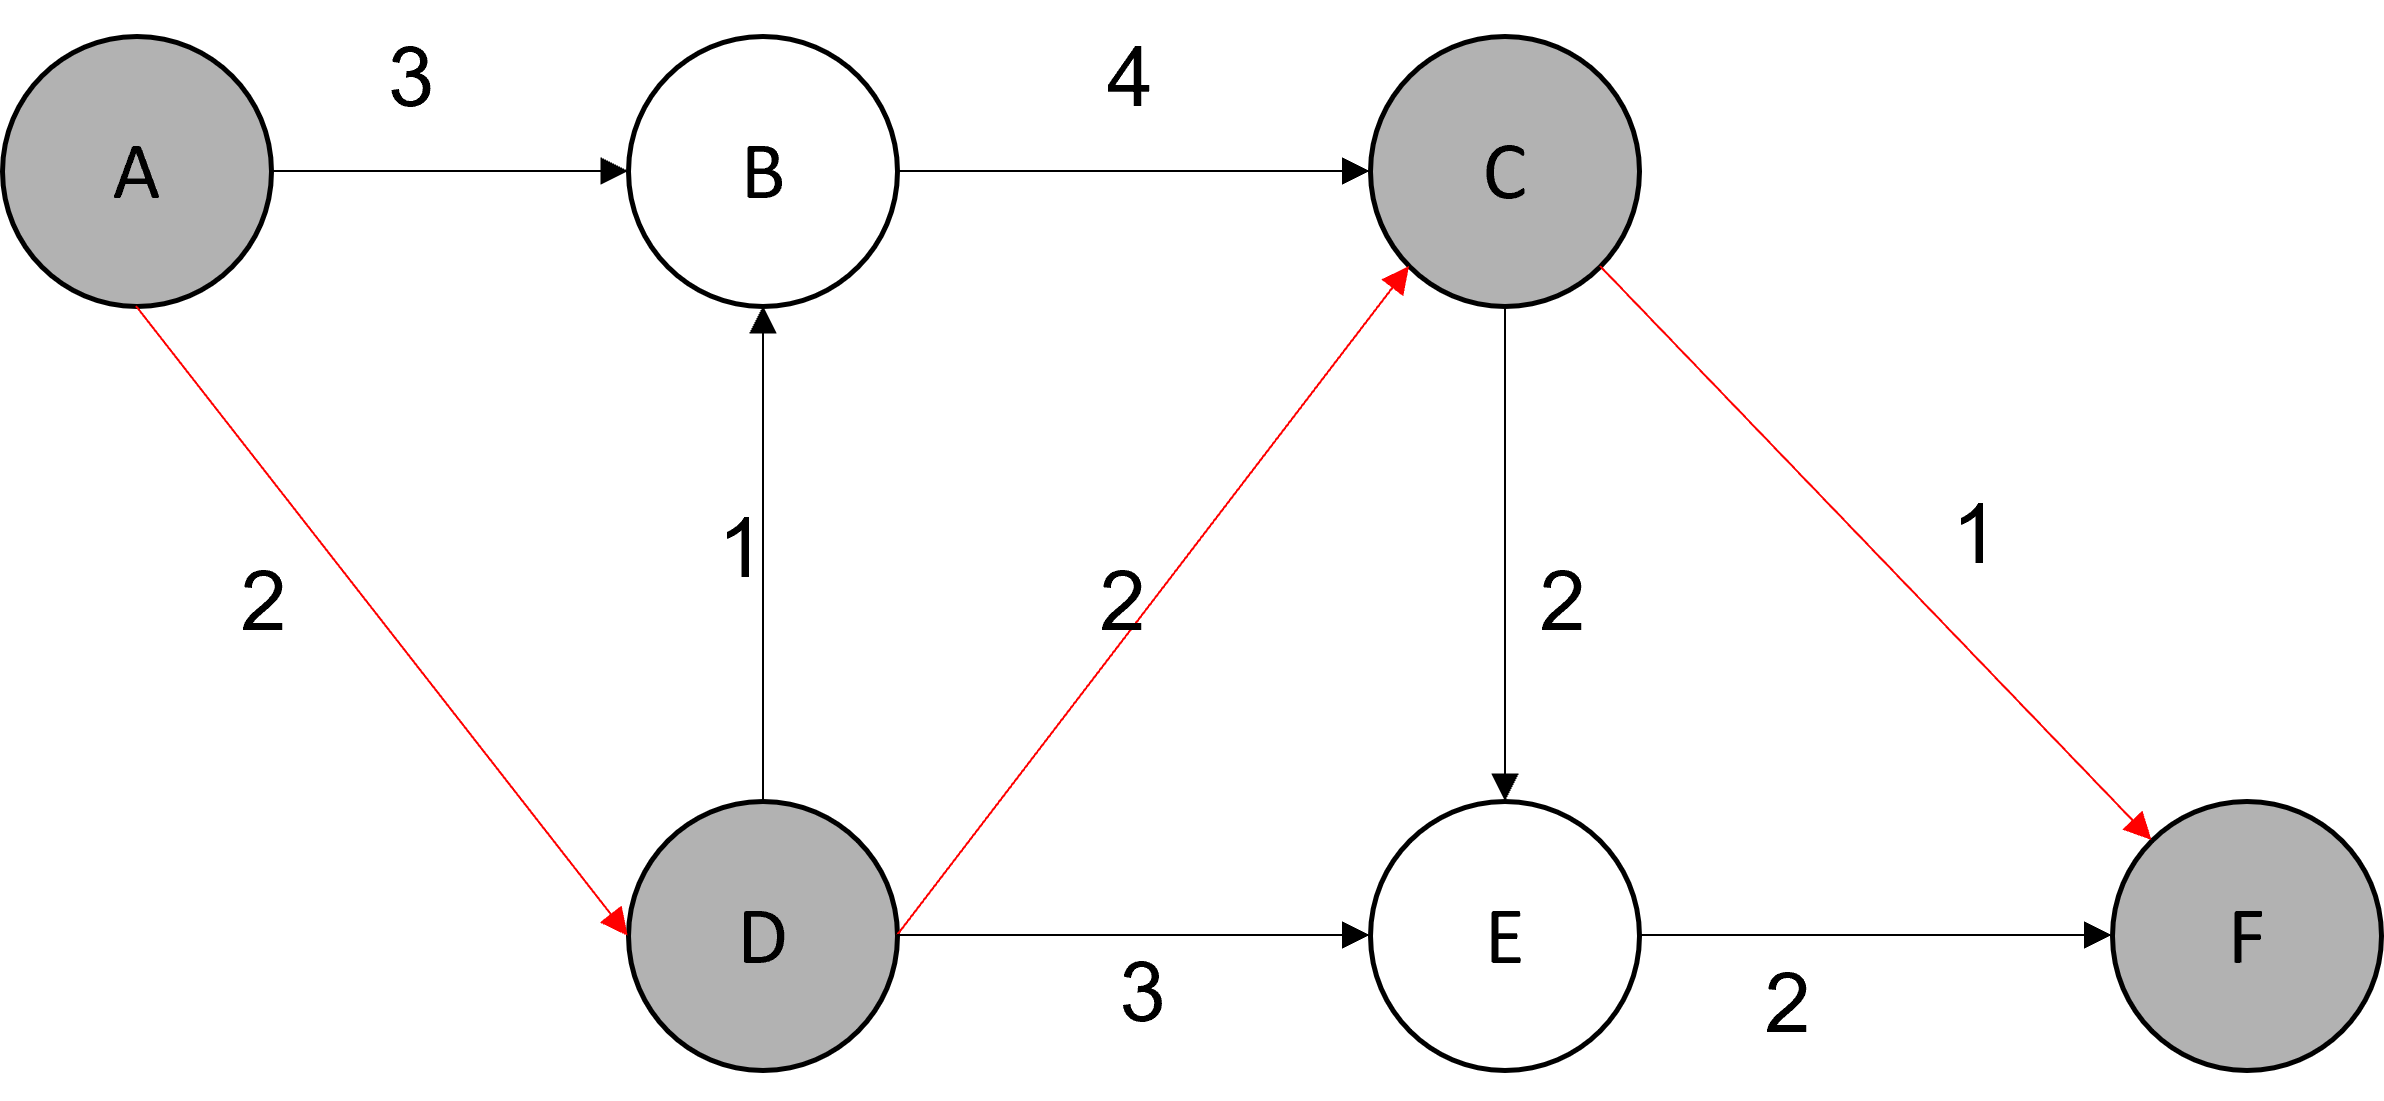
\includegraphics[width=0.6\textwidth]{png/图片18 最短路径A1} %插入图片,[]中设置图片大小,{}中是图片文件名
        \caption{最短路径$A^1$} %最终文档中希望显示的图片标题
        \label{fig:fig18} %用于文内引用的标签
    \end{figure}

    \item 将最短路径$A^1$中的所有路段添加到偏离点容器中,此时偏离点容器如图\ref{fig:fig19}所示
    \begin{figure}[H] %H为当前位置,!htb为忽略美学标准,htbp为浮动图形
        \centering %图片居中
        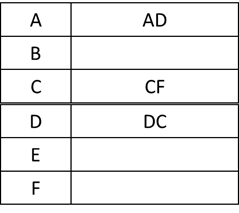
\includegraphics[width=0.45\textwidth]{png/图片18偏离点容器} %插入图片,[]中设置图片大小,{}中是图片文件名
        \caption{偏离点容器状态} %最终文档中希望显示的图片标题
        \label{fig:fig19} %用于文内引用的标签
    \end{figure}

    \item 依次以$A^1$中除汇点外的结点A,D,C作为偏离点,计算偏离路径,并添加到k最短路径的候选容器中,分别如图\ref{fig:fig20}
    \begin{figure}[htbp]
        \centering  %图片全局居中
        \subfigure[偏离路径$A_1^2$]{
            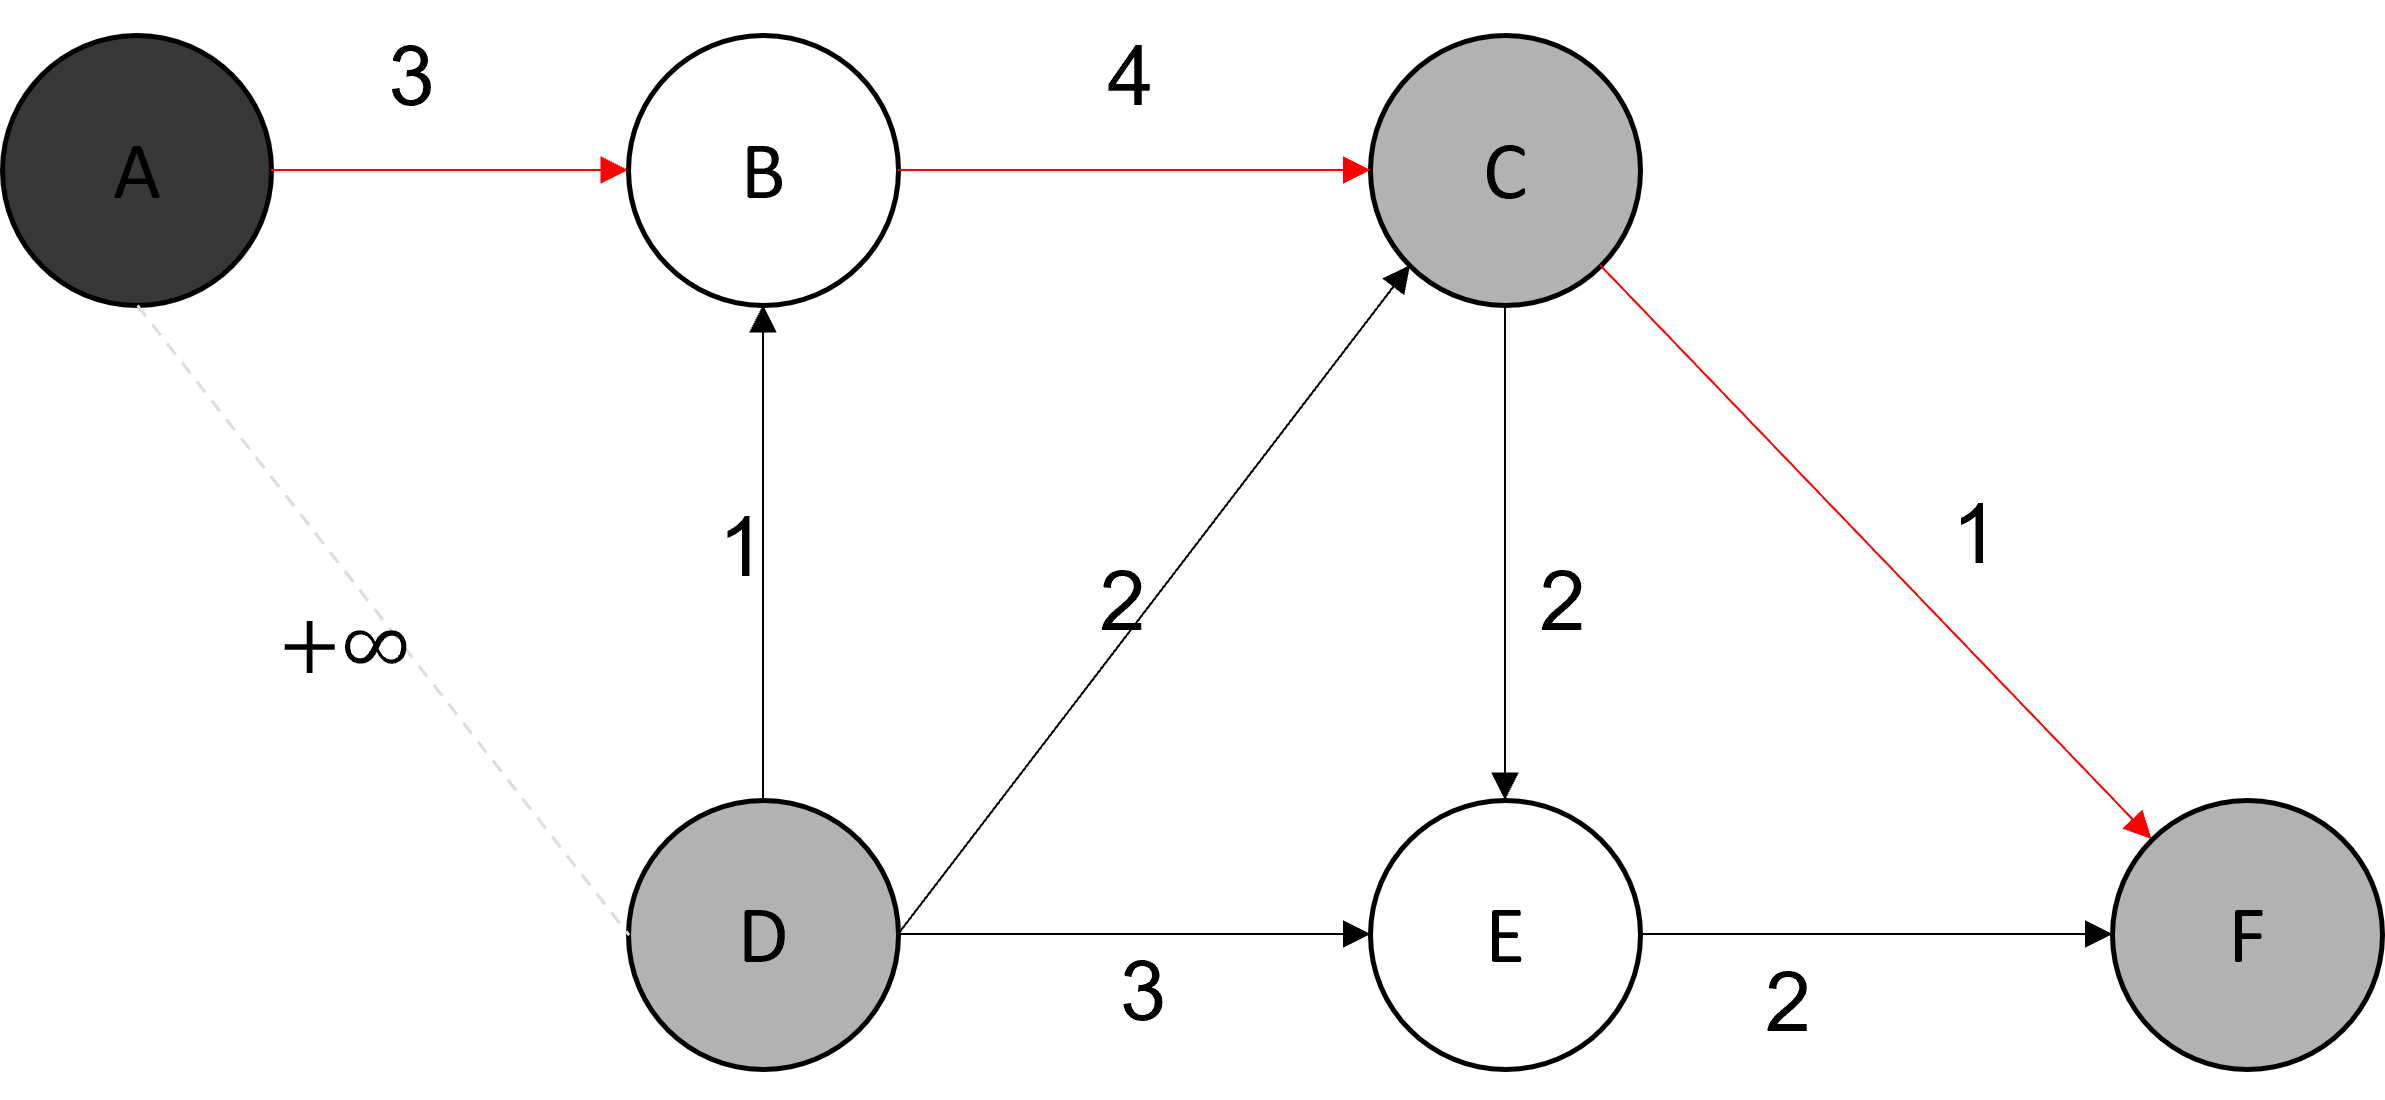
\includegraphics[width=0.45\textwidth]{png/图片19偏离路径A2_1的计算}}
        \quad
        \subfigure[偏离路径$A_2^2$]{
            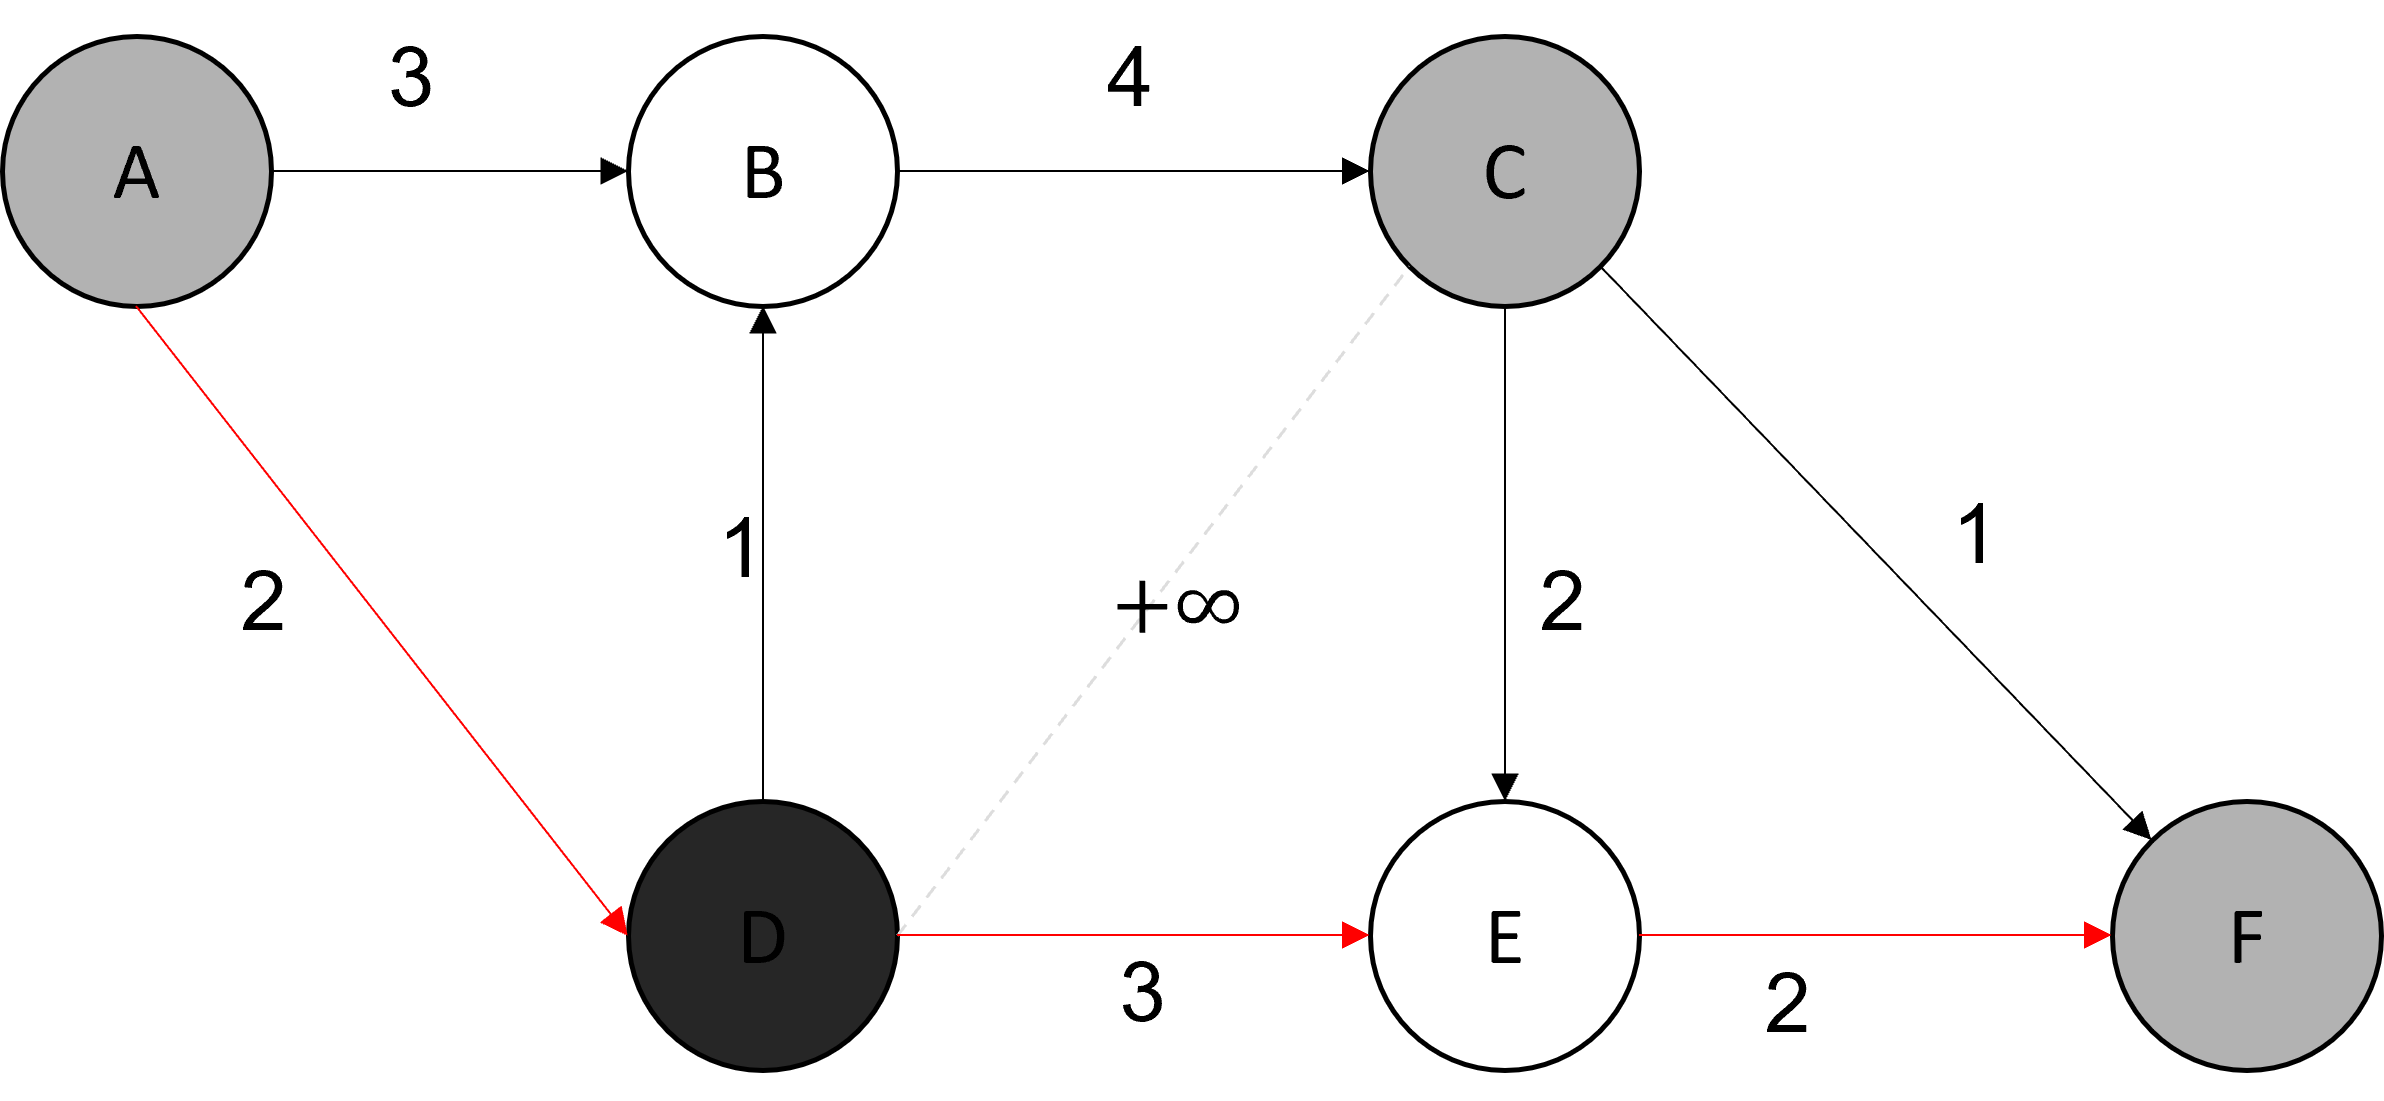
\includegraphics[width=0.45\textwidth]{png/图片20偏离路径A2_2的计算}}
        \quad
        \subfigure[偏离路径$A_3^2$]{
            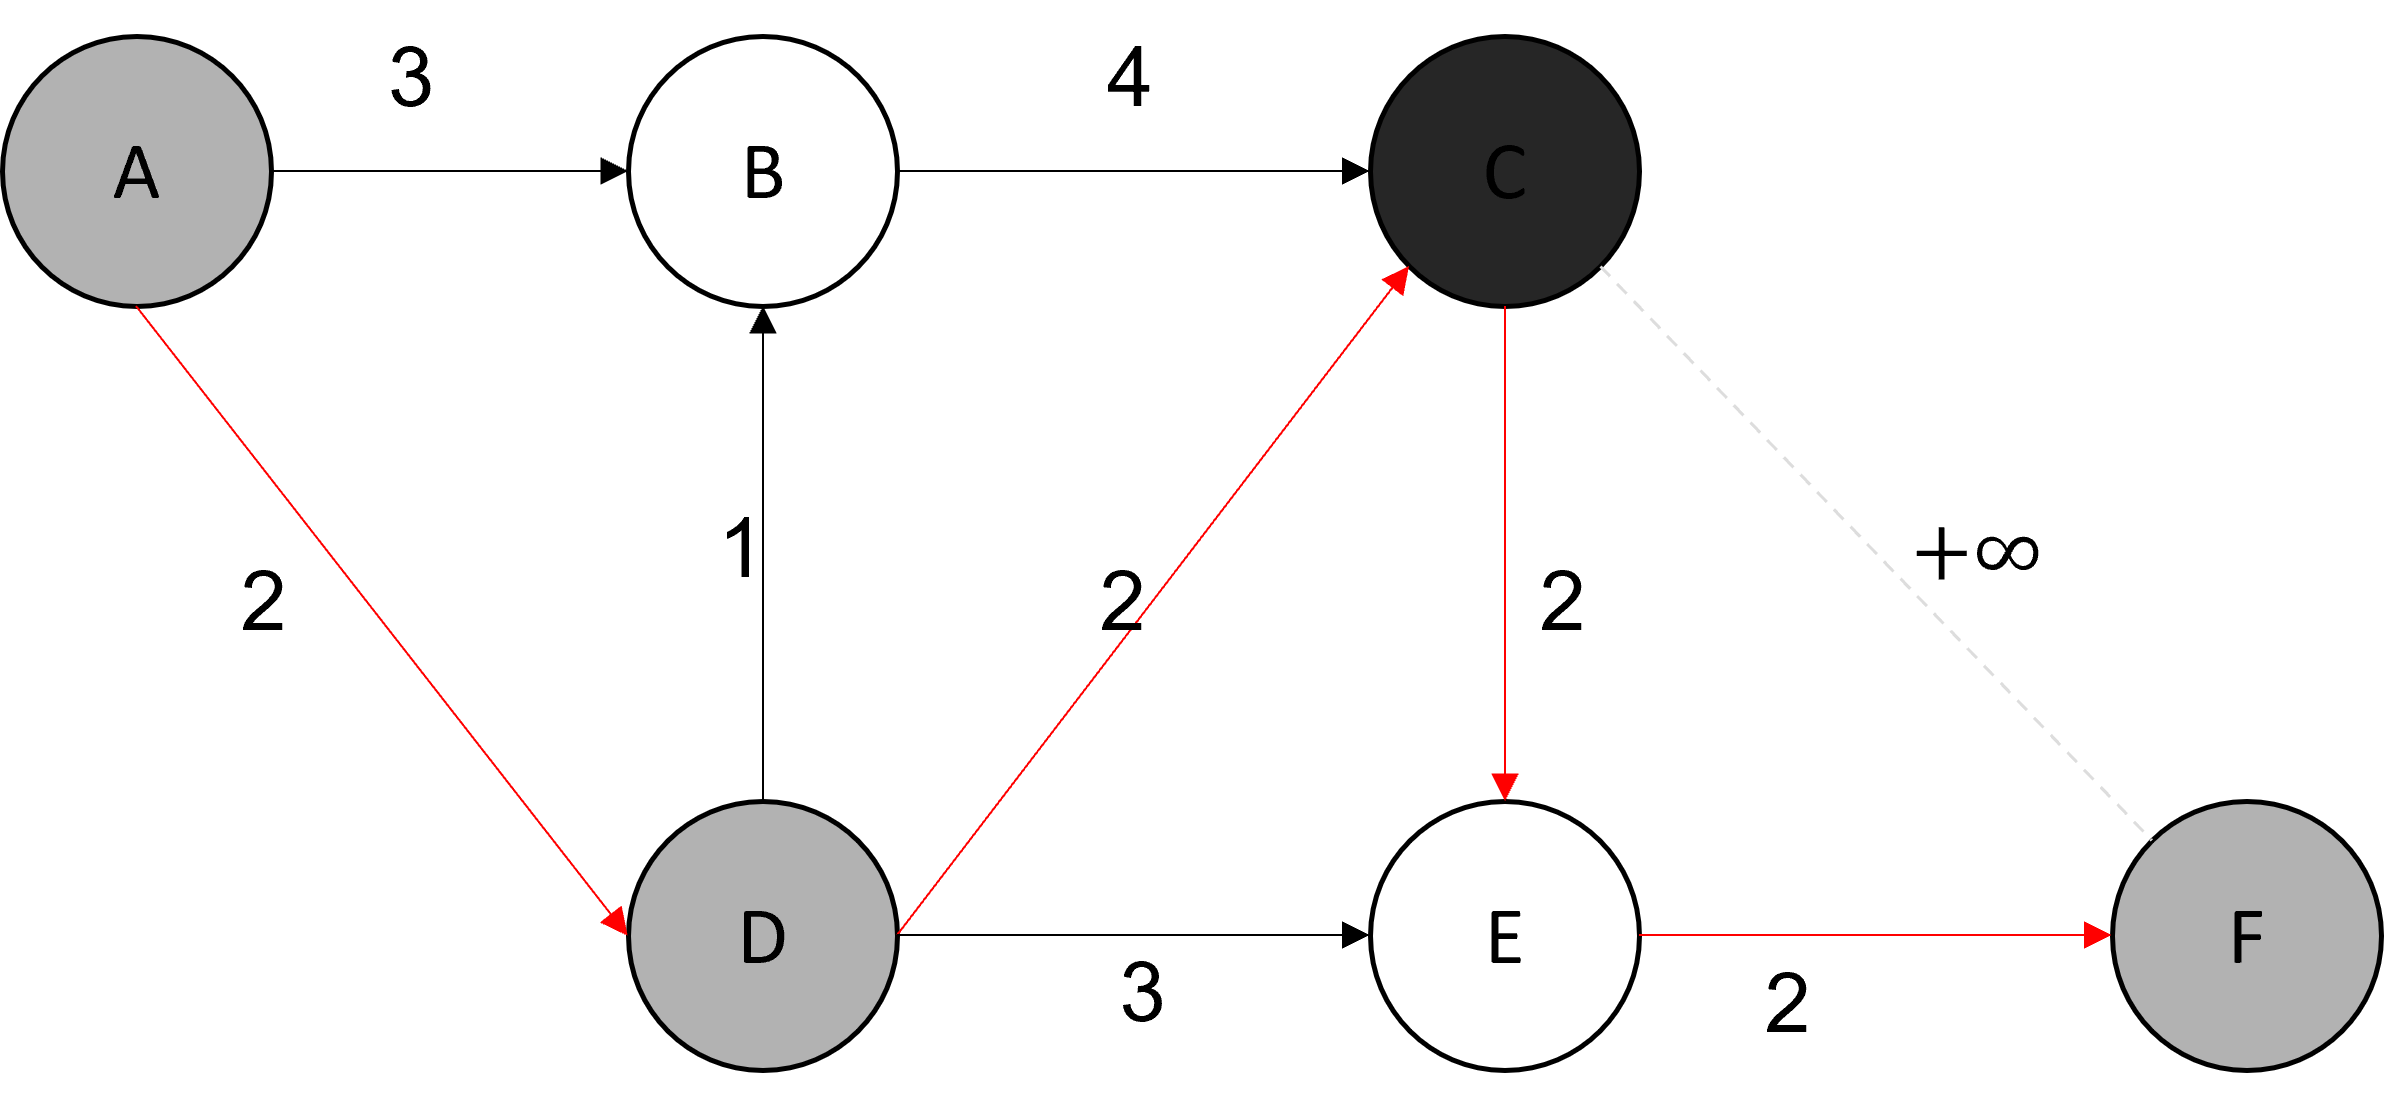
\includegraphics[width=0.45\textwidth]{png/图片21偏离路径A2_3的计算}}
        \quad
        \subfigure[最短路径$A^1$]{
            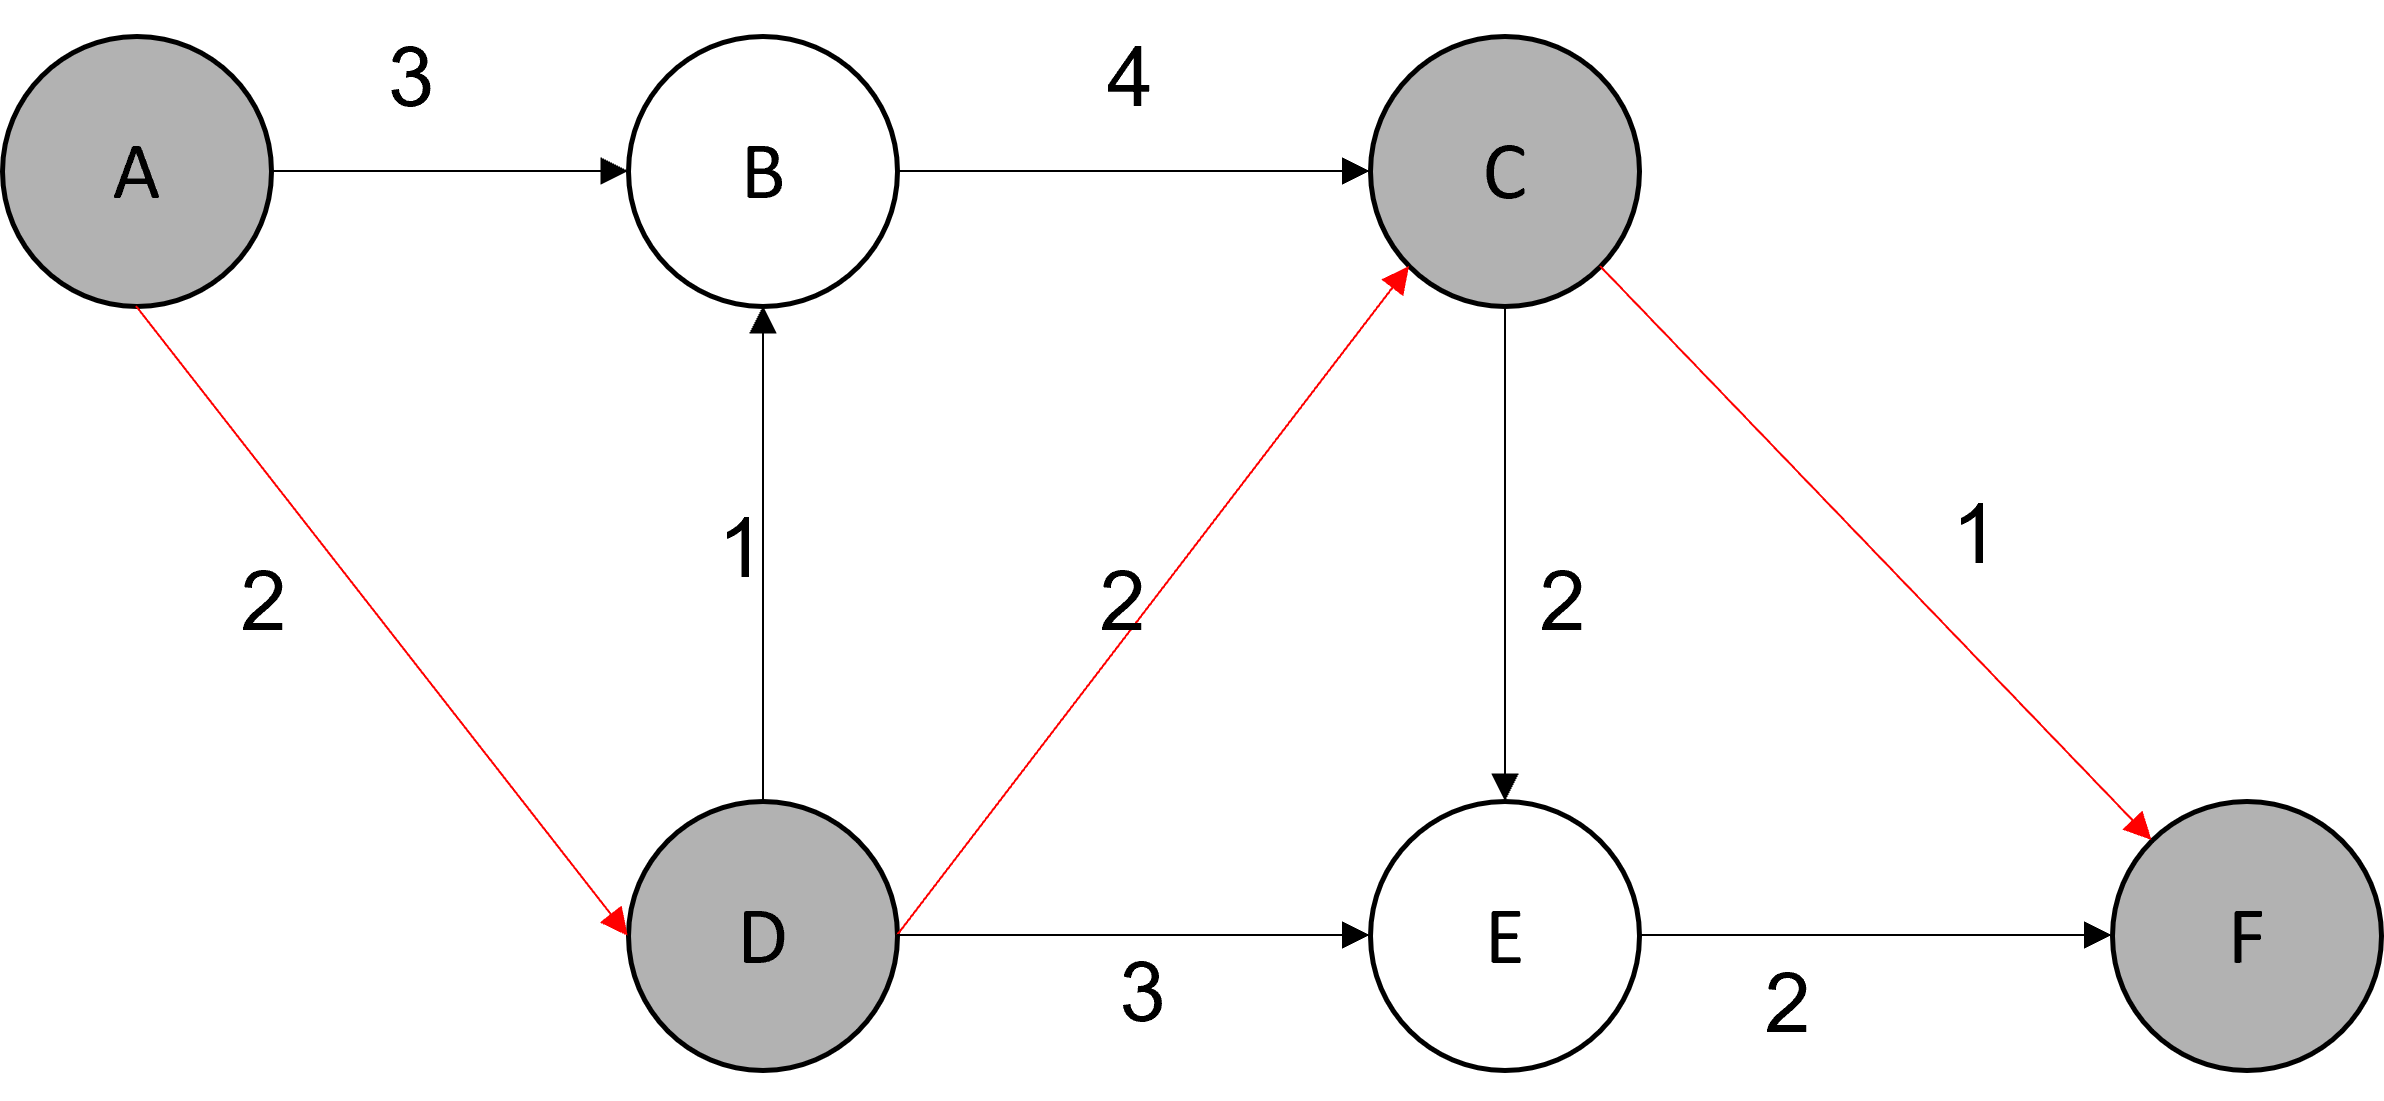
\includegraphics[width=0.45\textwidth]{png/图片18 最短路径A1}}
        \caption{偏离路径$A_i^2$的计算}
        \label{fig:fig20}
    \end{figure}

    \item 此时k最短路径候选容器状态如图\ref{fig:fig202}所示,从中选择最短的路径最为当前所求的k最短路径,显然此时最短路径为偏离路径$A_2^2$
    \begin{figure}[H] %H为当前位置,!htb为忽略美学标准,htbp为浮动图形
        \centering %图片居中
        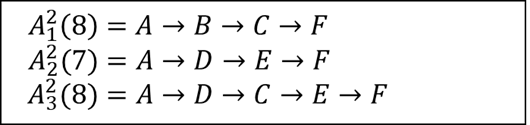
\includegraphics[width=0.7\textwidth]{png/图片20 k最短路径候选容器} %插入图片,[]中设置图片大小,{}中是图片文件名
        \caption{k最短路径候选容器} %最终文档中希望显示的图片标题
        \label{fig:fig202} %用于文内引用的标签
    \end{figure}

    \item 更新偏离点容器,容器状态如图\ref{fig:fig21}所示
    \begin{figure}[H] %H为当前位置,!htb为忽略美学标准,htbp为浮动图形
        \centering %图片居中
        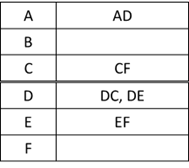
\includegraphics[width=0.45\textwidth]{png/图片21 更新偏离点容器} %插入图片,[]中设置图片大小,{}中是图片文件名
        \caption{更新偏离点容器} %最终文档中希望显示的图片标题
        \label{fig:fig21} %用于文内引用的标签
    \end{figure}

    \item 以A为偏离点,计算偏离路径$A_1^3$,如图\ref{fig:fig192}所示,发现此时$A_1^3=A\to B\to C \to F$已经出现在容器B中,因此不需要添加到容器之中;
    \begin{figure}[H] %H为当前位置,!htb为忽略美学标准,htbp为浮动图形
        \centering %图片居中
        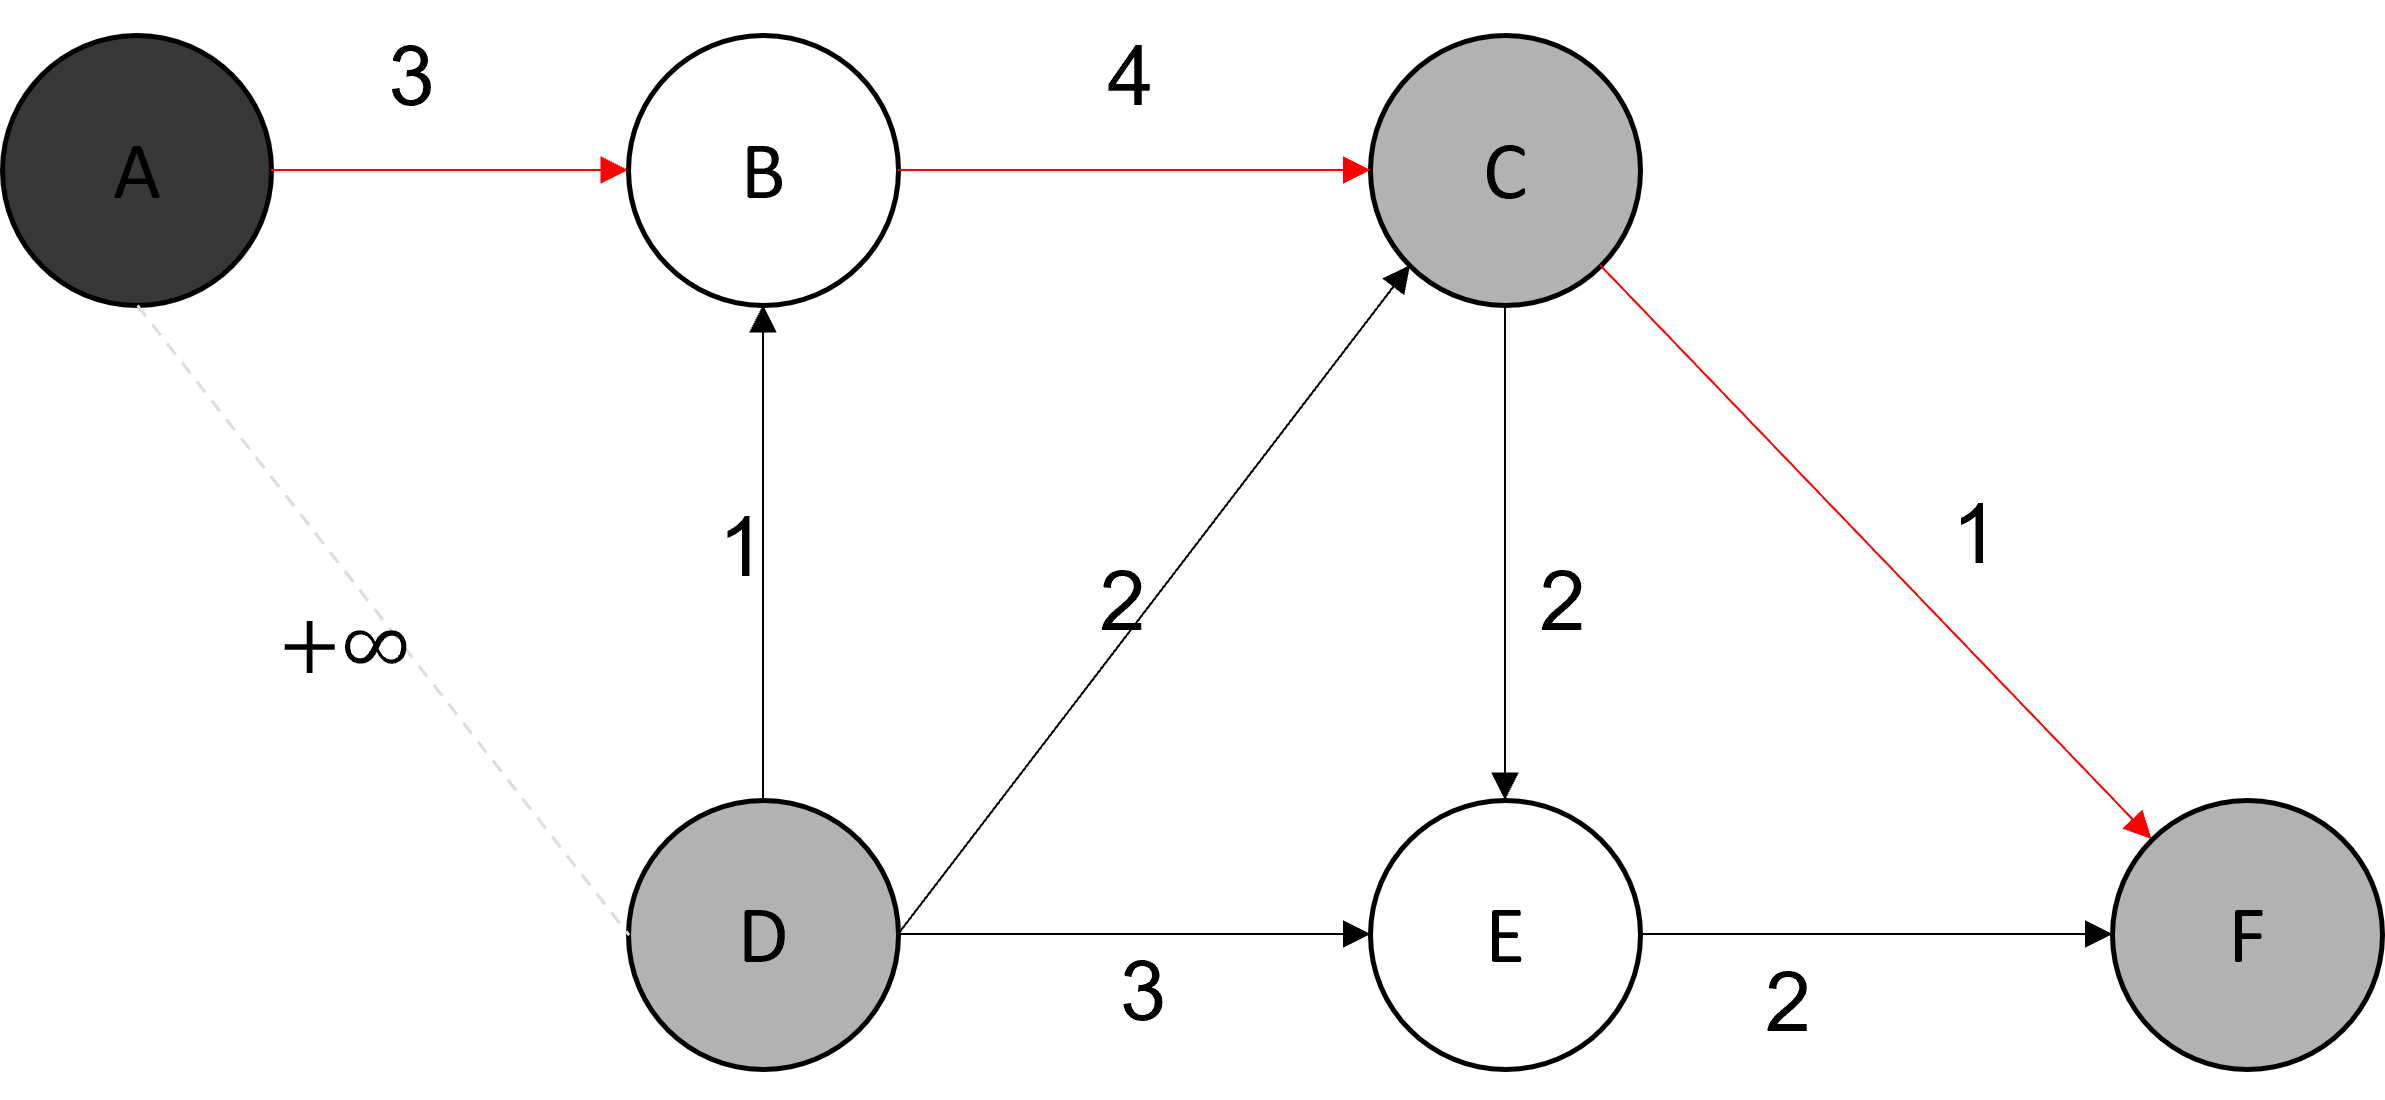
\includegraphics[width=0.7\textwidth]{png/图片19偏离路径A2_1的计算} %插入图片,[]中设置图片大小,{}中是图片文件名
        \caption{偏离路径$A_1^3$的计算} %最终文档中希望显示的图片标题
        \label{fig:fig192} %用于文内引用的标签
    \end{figure}

    \item 以D为偏离点,计算偏离路径$A_2^3(8)=A\to D\to B\to C\to F$,如图\ref{fig:fig27}所示,并添加到容器B中作为$A^3$的候选路径;
    \begin{figure}[H] %H为当前位置,!htb为忽略美学标准,htbp为浮动图形
        \centering %图片居中
        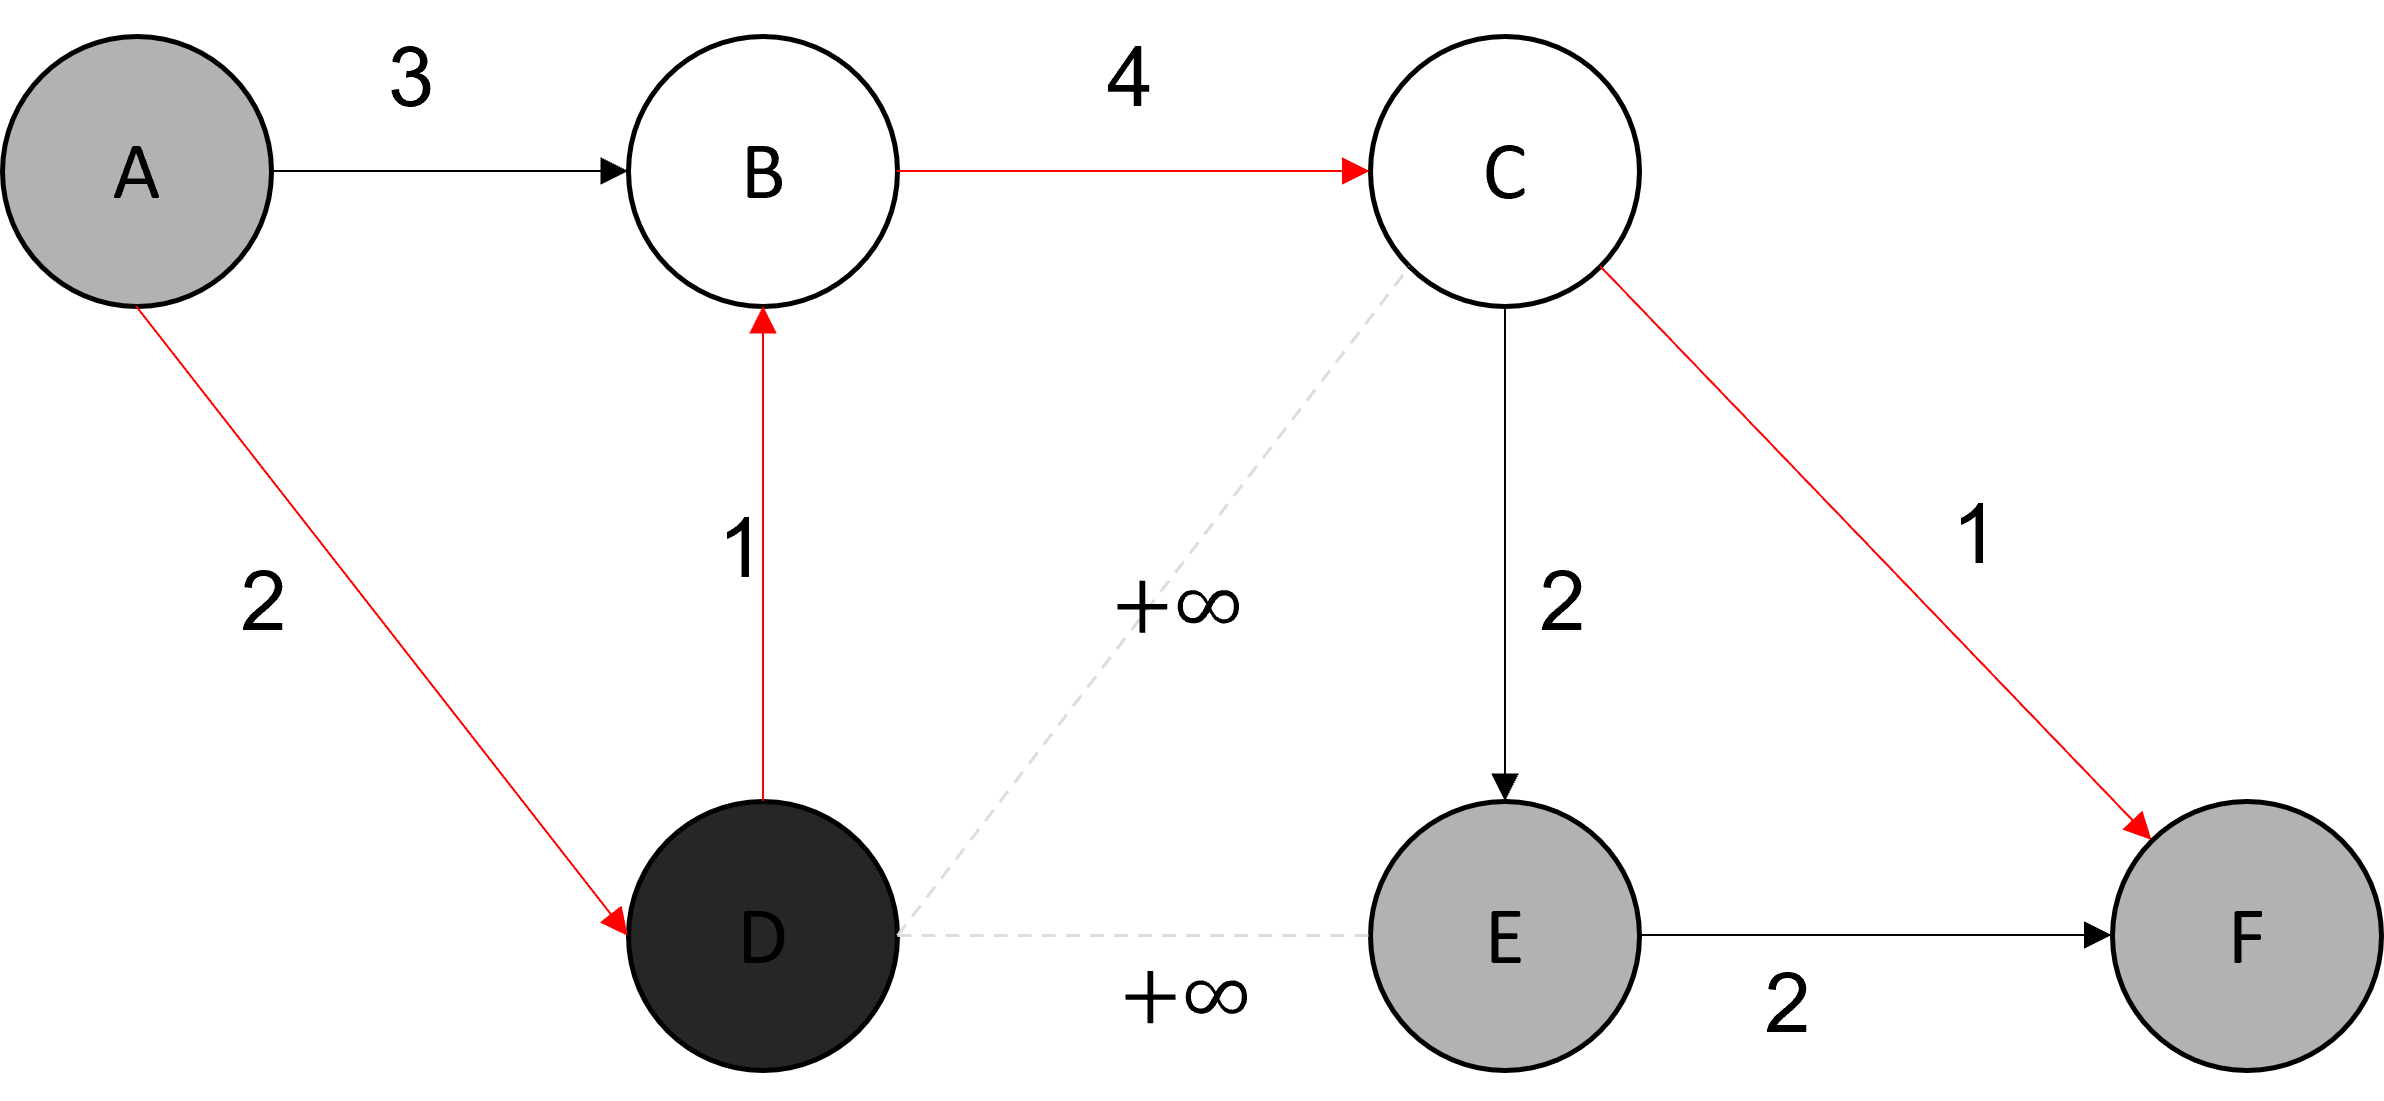
\includegraphics[width=0.7\textwidth]{png/图片27 偏离路径A3_2} %插入图片,[]中设置图片大小,{}中是图片文件名
        \caption{偏离路径$A^3_2$} %最终文档中希望显示的图片标题
        \label{fig:fig27} %用于文内引用的标签
    \end{figure}

    \item 以E为偏离点,计算偏离路径$A_3^3$,此时不存在以E为偏离点的偏离路径,如图\ref{fig:fig28}所示;
    \begin{figure}[H] %H为当前位置,!htb为忽略美学标准,htbp为浮动图形
        \centering %图片居中
        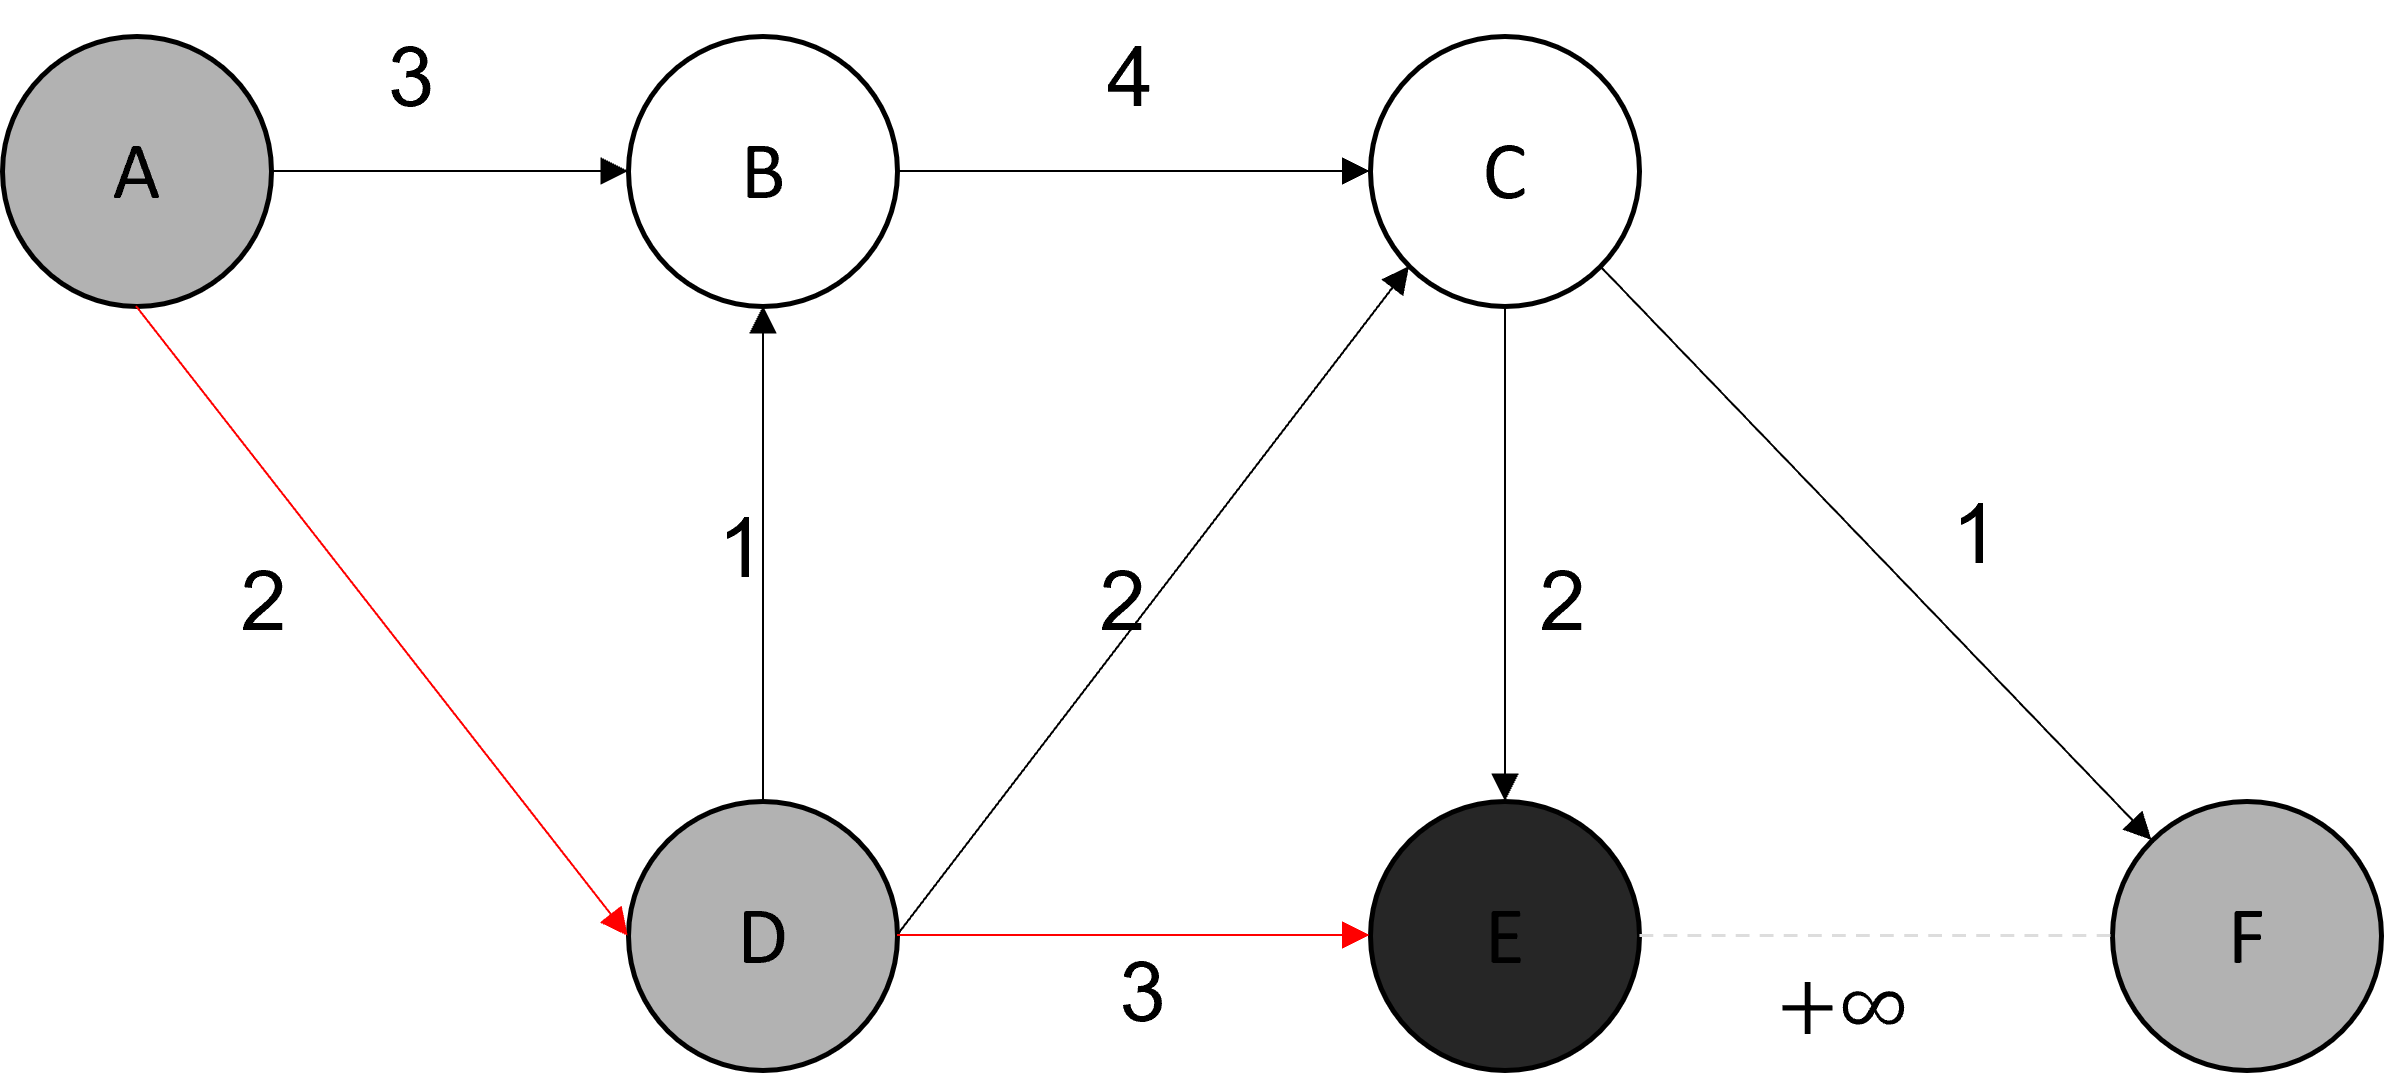
\includegraphics[width=0.7\textwidth]{png/图片28 不存在偏离路径A3_3} %插入图片,[]中设置图片大小,{}中是图片文件名
        \caption{不存在偏离路径$A^3_3$} %最终文档中希望显示的图片标题
        \label{fig:fig28} %用于文内引用的标签
    \end{figure}

    \item 从容器B取出最短路径,即$A^3=A\to D\to B\to C\to F$,自此算法执行完毕。
\end{enumerate}


\section{程序正确性验证}\label{sec:程序正确性验证}

\begin{figure}[H] %H为当前位置,!htb为忽略美学标准,htbp为浮动图形
    \centering %图片居中
    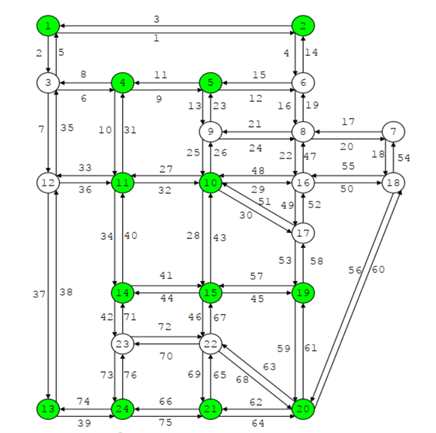
\includegraphics[width=0.7\textwidth]{png/图片22 SiouxFall测试网络} %插入图片,[]中设置图片大小,{}中是图片文件名
    \caption{SiouxFall测试网络} %最终文档中希望显示的图片标题
    \label{fig:fig22} %用于文内引用的标签
\end{figure}
分别对上述简单测试网络和如图\ref{fig:fig22}所示的Sioux Falls测试网络执行k最短路程序,对于SiouxFall测试网络输出前10条最短路如表\ref{tab:table1}所示,程序执行效果分别如图\ref{fig:fig23}, 图\ref{fig:fig24}所示。
程序运行结果和手工计算得到的结果完全相同,可以说明k最短路程序的正确性,因此下一章节将会将该程序用于规模更大、情况更加复杂的实际城市道路网络模拟中。
\begin{table}[H]
    \begin{center}
        \caption{SiouxFalls网络前10条无环最短路径及代价}\label{tab:table1}
        \begin{tabular}{ll}
            \hline
            最短路径                                                                                                                                                    & 路径成本 \\
            \hline
            $A^1= 1 \rightarrow 3 \rightarrow 12 \rightarrow 24$                                                                                                    & 85   \\
            $A^2= 1 \rightarrow 2 \rightarrow 6 \rightarrow 5 \rightarrow 4 \rightarrow 3 \rightarrow 12 \rightarrow 13 \rightarrow 24$     & 122  \\
            $A^3= 1 \rightarrow 3 \rightarrow 4 \rightarrow 11 \rightarrow 12 \rightarrow 13 \rightarrow 24$     & 127  \\
            $A^4= 1 \rightarrow 3 \rightarrow 4 \rightarrow 11 \rightarrow 14 \rightarrow 13 \rightarrow 24$     & 131  \\
            $A^5= 1 \rightarrow 2 \rightarrow 6 \rightarrow 5 \rightarrow 4 \rightarrow 11 \rightarrow 12 \rightarrow 13 \rightarrow 24$     & 150  \\
            $A^6= 1 \rightarrow 2 \rightarrow 6 \rightarrow 5 \rightarrow 4 \rightarrow 11 \rightarrow 14 \rightarrow 13 \rightarrow 24$     & 154  \\
            $A^7= 1 \rightarrow 3 \rightarrow 12 \rightarrow 11 \rightarrow 14 \rightarrow 13 \rightarrow 24$     & 158  \\
            $A^8= 1 \rightarrow 2 \rightarrow 6 \rightarrow 8 \rightarrow 9 \rightarrow 5 \rightarrow 4 \rightarrow 3 \rightarrow 12 \rightarrow 13 \rightarrow 23$     & 167  \\
            $A^9= 1 \rightarrow 3 \rightarrow 4 \rightarrow 11 \rightarrow 14 \rightarrow 23 \rightarrow 24$     & 167  \\
            $A^{10} = 1 \rightarrow 2 \rightarrow 6 \rightarrow 5 \rightarrow 4 \rightarrow 11 \rightarrow 14 \rightarrow 23 \rightarrow 24$ & 190  \\
            \hline
        \end{tabular}
    \end{center}
\end{table}

\begin{figure}[H] %H为当前位置,!htb为忽略美学标准,htbp为浮动图形
    \centering %图片居中
    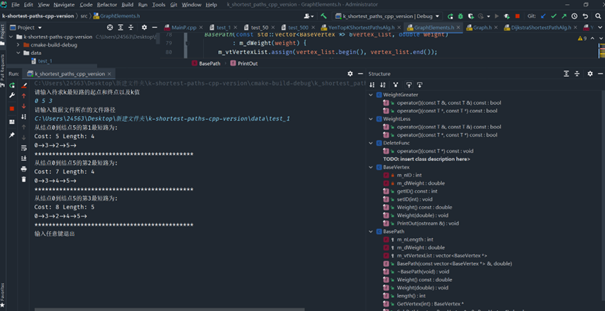
\includegraphics[width=0.9\textwidth]{png/图片23 6结点测试网络执行结果} %插入图片,[]中设置图片大小,{}中是图片文件名
    \caption{6结点测试网络执行结果} %最终文档中希望显示的图片标题
    \label{fig:fig23} %用于文内引用的标签
\end{figure}

\begin{figure}[H] %H为当前位置,!htb为忽略美学标准,htbp为浮动图形
    \centering %图片居中
    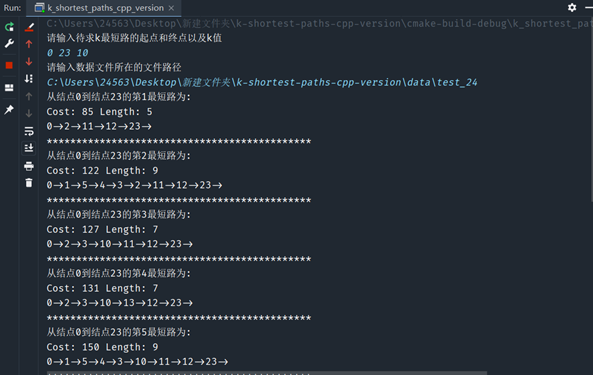
\includegraphics[width=0.9\textwidth]{png/图片24 SiouxFall测试网络执行结果} %插入图片,[]中设置图片大小,{}中是图片文件名
    \caption{SiouxFall测试网络执行结果} %最终文档中希望显示的图片标题
    \label{fig:fig24} %用于文内引用的标签
\end{figure}


\section{程序效率分析}\label{sec:程序效率分析}
在Sioux Falls测试网络程序可以很快的得到输出结果,之后对更大规模随机生成初始数据的网路进行程序的执行效率测试。
测试环境为Intel(R) Core(TM) i5-8300H CPU @ 2.30GHz和16GB的RAM,
测试在结点数和路段数分别在(a)24个结点50条路段、(b)50个结点1600条路段、(c)500个结点5800条路段、(d)800个结点8800条路段、(e)1000个结点11000条路段,
重复进行10次实验取平均值后统计程序执行时间,考虑到文件输入输出时间的不同,因此不包括文件的输入输出时间,程序执行时间结果如图\ref{fig:fig32}所示,可以发现程序执行时间大致随着边数呈现线性分布。
\begin{figure}[H] %H为当前位置,!htb为忽略美学标准,htbp为浮动图形
    \centering %图片居中
    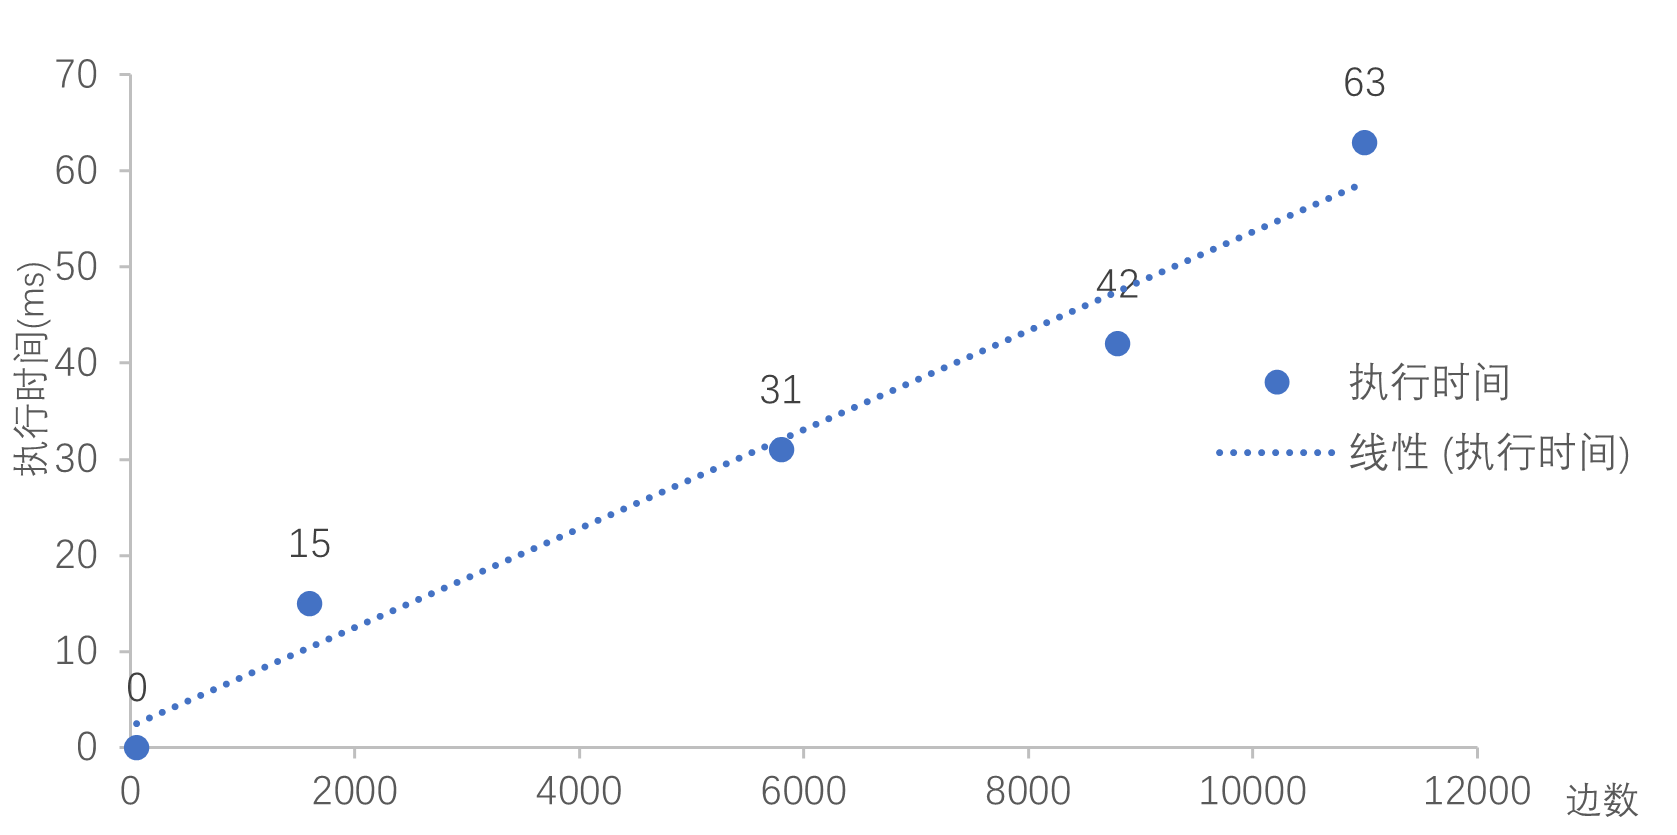
\includegraphics[width=0.7\textwidth]{png/图片32 程序执行时间与网络规模之间的关系} %插入图片,[]中设置图片大小,{}中是图片文件名
    \caption{程序执行时间与网络规模之间的关系} %最终文档中希望显示的图片标题
    \label{fig:fig32} %用于文内引用的标签
\end{figure}


\section{可靠性分析}\label{sec:可靠性分析}
可靠性是指在规定的条件下和规定的时间内,完成规定功能的能力。
在实际出行需求中,除考虑到出行者的距离花费和时间花费外,在特殊的场景中,往往还存在着可靠性要求。以常见的高铁出行方式中,出行者往往需要在特定的时间前到达高铁站,此时可能并不关注具体花费多长时间,而是需要赶在高铁出发前到达,类似这种应用场景下,路径可靠性要求将起到决定性的作用。
对道路系统而言,可靠度越高就越好。可靠度高的道路系统,可以长时间正常工作(这正是所有出行者需要得到的)。此外,高可靠性的道路系统还可以提供一定的道路故障容错,不会因为某条路段的道路维护造成行程时间的大幅度增加并对预计行程计划造成严重影响。

可靠度一般可分成两个层次,首先是所谓组件可靠度(Reliability of component)。也就是将产品拆解成若干不同的零件或组件,先就这些组件的可靠度进行研究,然后再探讨整个系统、整个产品的整体可靠度,也就是系统可靠度(Reliability of system)。
可靠度的概念不仅仅局限在交通系统中,但在交通系统中,可靠度可进一步划分。例如,组件可靠度可以进一步细分为连通可靠度和旅行时间可靠度,而系统可靠度则对应路网容量可靠度。

\subsection{出行时间可靠性分析}\label{subsec:出行时间可靠性分析}
驾驶者出行前通常都会估计正常情况下的行程时间,一般会选择提早出发时间来给道路系统提供一定的容错时间,但是出行时间不可能无限制的提前,因此对道路系统的可靠性作出相应的要求,可靠度的提高是反映交通管理效果的重要方面。此外,在考虑出行时间的可靠性的同时需要结合路网实际饱和度,路网容量,出行阻抗等因素综合考虑。出行时间可靠性是交通网络的随机性,路网运行的实际状态和驾驶者的决策行为共同作用的结果。通过路径诱导系统发布多条路线的行程时间和可靠性信息,可以有效地影响驾驶者的决策行为。

\subsection{连通可靠度分析}\label{subsec:连通可靠度分析}
行程时间可靠度的影响因素可能有如下方面:车辆抛锚,交通事故,交通信号灯,公交停靠站,车辆合流分流,交通流中大型车的比例,公路铁路交叉口的等待时间等。出行者会在自己的出行预算中增加一个预算时间,达到最终平衡。

可靠度的分类:连通可靠度,旅行时间可靠度,路网容量可靠度
\begin{itemize}%无序列表
    \item \textbf{连通可靠度}\\
    关注于网络拓扑结构的连通情况,关注网络中od对之间是否至少存在一条可行路径连通。而路段连通与否有两种状态:连通和不连通,分别使用1和0进行表示。
    在路段被破坏或维护时,可以认为路段不连通,或者当路段的交通流量是否超过路段容量,超过则认为不连通,此外还有学者提出当路段的交通流量超过某个阈值时可认为路段处于不连通的状态,这个阈值可以是某个固定值,可以是道路的初始容量,也可以是某个小于1的系数和道路容量的乘积。

    \item \textbf{旅行时间可靠度}\\
    在给定的时间间隔和要求的服务水平下,从指定出发点到指定目的地之间能够达到的概率。 可以用路段阻抗函数在给定时间间隔下的时间宽度比上总的时间长度。旅行时间可靠度本质上反映了行程时间的动态性和不确定性。

    \item \textbf{容量可靠度}\\
    在给定服务水平下网络容量能够适应一定交通需求的概率。
    交通网络中路段容量是会受到各种诸如时间,气候因素,天气状况,突发事件等各种不确定因素的影响而不断变化。交通网络的参与对象是人,具有一定的能动性和主观情感,不像其它货物,交通网络中的拥挤回由于拥挤产生延误,交通网络中的容量会受到路段容量,交通需求水平,拥挤,驾驶者的路径决策等的影响。
\end{itemize}


